\chapter{Approach}\label{chapter:approach}
Approach

\section{Lazy Logging}

\subsection{Prerequisites}

\subsection{Design and Architecture}

\subsection{Implementation}

\section{Block size limit}
The introduction of a block size limit allows a more accurate simulation of the Bitcoin network.

\subsection{Prerequisites}

\subsection{Design and Architecture}

\subsection{Implementation}

\section{Alternative history attack}

\subsection{Prerequisites}

To simulate an alternative history attack additional \textbf{configuration parameters} are necessary. These parameters are used for the actual simulation of the attack, the calcuation of the success probability of the attack and the maximum safe transaction value.

\begin{itemize}
\item \textit{isAlternativeHistoryAttack}: if an alternative history attack is simulated as a boolean
\item \textit{hashrate}: attacker's hashrate as a percentage of the total hashrate of the Bitcoin Network
\item \textit{confirmations}: the amount of confirmations the attacked merchants are waiting for to accept a transaction
\item \textit{attackDuration}: the attacker gives up after mining a certain amount of blocks and not suceeding or if it is not possible anymore to surpass the level of the public blockchain
\item \textit{discountOnStolenGoods}: discount of the stolen goods by the attacker, a value from 0 (= full discount) to 1 (= no discount)
\item \textit{amountOfAttackedMerchants}: the attack is carried out against a certain amount of merchants at the same time
\item \textit{blockReward}: current block reward in BTC
\end{itemize}

\subsection{Design and Architecture}

\subsubsection{Simulating the attack}

In the following the attacker's nodes, blockchain or blocks are interchangeably described as \textit{evil} and the public networks' nodes as \textit{good}.\linebreak

The solution for the simulation of an alternative history attack selects nodes as attacking nodes according to the attacker's hashrate as a percentage of the total Bitcoin Network.
The good and the evil nodes both can mine the genesis block. The genesis block is then the first block in both the good and the evil blockchain. For simplicity we assume that the attacker successfully sent the transactions to the attacked merchants in the second block of the public blockchain. Immediately after the genesis block is mined, the evil nodes start mining together on their own evil blockchain. It is necessary for all nodes to update their neighbour nodes to only have their corresponding nodes as neighbours. For example in the case of a low amount of evil nodes and a low amount of neighbours... Since the attacker of course doesn't want his...\linebreak

Finally the success of the simulated attack is decided if the attacker's blockchain level can surpass the public's blockchain level after waiting for the Merchants confirmation and before the attack duration ends.

\subsubsection{Calculating the success probability  \cite{doublespending}}

Before the formula to calculate the success probability of an alternative history attack is shown, the variables need to be defined.\linebreak
...

\begin{equation}
p + q = 1
\end{equation}

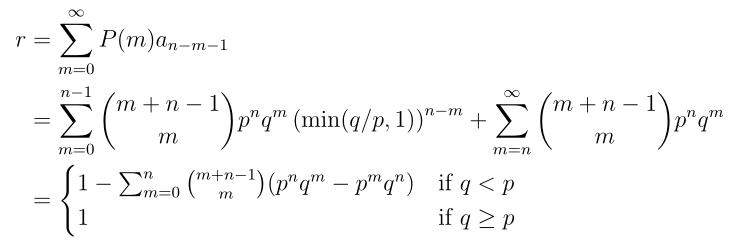
\includegraphics[scale=0.7]{successProbability.PNG} 

The formula for $q < p$ is transformed to the following formula to be used in the implementation.

\begin{equation}
r = 1-\sum\limits_{m=0}^n \frac{(m+n-1)!}{m!\,(n-1)!}(p^nq^m-p^mq^n)
\end{equation}

\subsubsection{Calculating the safe transaction value  \cite{doublespending}}

\begin{equation}
k \alpha v - (1 - r)(kv + oB) = kv( \alpha + r - 1) - (1 - r)oB
\end{equation}

\subsection{Implementation}



VConf ...

\begin{minipage}{\linewidth}
\begin{lstlisting}[style=myScalastyle]
object VBlock extends LazyLogging {
  def createWinnerBlock(node: VNode, timestamp: DateTime): VBlock = {
    var maxTransactionsPerBlock : Int = 0
    var processedTransactionsInBlock: Set[VTransaction] = Set.empty

    if (VConf.strategy == "BITCOIN_LIKE_BLOCKCHAIN") {
      // todo think about if to implement SegWit (maxBlockWeight vs maxBlockSize)
      maxTransactionsPerBlock = Math.floor(VConf.maxBlockSize / VConf.transactionSize).toInt

      // sorts the transaction pool by the transaction fee
      processedTransactionsInBlock = node.transactionPool.toSeq.sortWith(_.transactionFee > _.transactionFee).take(maxTransactionsPerBlock).toSet

      // sets confirmation status of transaction true
      processedTransactionsInBlock.foreach { _.confirmation = true }

      // sets confirmation level of transaction
      processedTransactionsInBlock.foreach { _.confirmationLevel = node.blockchain.size }
    } else {
      maxTransactionsPerBlock = node.transactionPool.size
      processedTransactionsInBlock = node.transactionPool
    }

    VBlock(
      id = UUID.randomUUID().toString,
      origin = node,
      transactions = processedTransactionsInBlock,
      level = node.blockchain.size,
      timestamp = timestamp,
      recipients = ListBuffer.empty,
      transactionPoolSize = node.transactionPool.size
    )
  }
}
\end{lstlisting}
\end{minipage}